%07/11 - Estrella
\chapter{Bases de datos no relacionales}
\section{Bases de datos no SQL}
Una base de datos es un conjunto de datos interrelacionados. Los datos registran eventos significativos de cualquier tamaño y diferentes grados de complejidad. Para gestionar las bases de datos, hay sistemas de gestión de bases de datos (SGBD). Se trata de un software que permite \textit{definir los datos a almacenar} (especificando el tipo de datos, su estructura y restricciones), \textit{construir la base de datos para almacenar la información} y \textit{manipular los datos} (consultar los datos, actualizarlos y generar informes). Por ejemplo, en el caso de una base de datos para la universidad, se tendría que especificar la estructura de los datos: 5 ficheros relativos a estudiantes, asignaturas, notas, requerimientos y grupos. Se debe especificar la estructura de cada una de las tablas y los tipos de datos para cada campo. Una vez hecho eso, se va guardando los datos en cada una de las tablas. Finalmente, se pueden manipular los datos para obtener los resultados a la lista de notas del estudiante Pérez, obtener los estudiantes registrados en la asignatura X, generar un nuevo grupo de la asignatura, etc. Las bases de datos relacionales se pueden representar gráficamente mediante modelos entidad-relación y modelos relacionales. La participación total se distingue de la parcial mediante puntas de flecha rellenas o vacías respectivamente. De igual forma, puede haber una o dos puntas de flecha para diferenciar las relaciones a uno y a muchos.

El sistema de gestión de bases de datos también debe asegurar la persistencia de datos, es decir, almacenar los datos de forma segura, mantener la consistencia de los datos (si alguna persona la modifica, que se actualice para todas las demás personas) y asegurar la disponibilidad de los datos mediante copias de seguridad.

\subsection{Motivación para las bases de datos no SQL}
Las bases de datos no SQL tienen cuatro razones principales:
\begin{itemize}
\item \textbf{Escalabilidad:} se define como escalabilidad vertical el cambio de un ordenador o servidor a otro más potente. La desventaja es que se debe parar la base de datos puntualmente durante la migración del sistema. La alternativa es la escalabilidad horizontal, es decir, formar una red de varios ordenadores o servidores conectados.
\item \textbf{Coste:} las bases de datos tradicionales funcionan mediante licencias basadas en el número de usuarios. En el caso de las aplicaciones web, no se puede estimar el número de usuarios que van a acceder a la base de datos a todas horas. Los sistemas de gestión de noSQL son de código abierto y, por tanto, gratuitos.
\item \textbf{Flexibilidad:} las bases de datos relacionales dependen de un buen diseño de tablas y columnas desde el principio. Además, todas las filas de la tabla tienen las mismas columnas, lo que en algunos casos puede ser un desperdicio de espacio si muchos campos se deben mantener vacíos (por ejemplo, en el caso de comercios online que venden una gran variedad de productos, cada uno con características diferentes).
\item \textbf{Disponibilidad}
\end{itemize}

Las bases de datos tradicionales o relacionales siguen un modelo ACID: atomicidad, consistencia, aislamiento y durabilidad. La atomicidad hace referencia a operaciones indivisibles, obligando a que se ejecuten todos los pasos o ninguno. La base de datos no se puede dejar en un estado en el que se viole la integridad de los datos; debe ser consistente. Además, las transacciones no son visibles a otros usuarios hasta que la ejecución se haya completado, siendo así operaciones aisladas. Finalmente, los datos deben estar guardados en un medio persistente para que tenga una gran durabilidad. 

Las bases de datos no SQL siguen un modelo BASE: básicamente disponibles, estado suave (soft state) y eventualmente consistente. Como las bases de datos siempre están en una red de servidores, están protegidos de fallos parciales. Los servidores vecinos se pueden hacer cargo de las tareas de un servidor, permitiendo que los datos estén disponibles. En algunos casos, las bases de datos pueden estar en un estado inconsistente, pero entonces se activa el proceso de replicación. El estado suave hace referencia a que el estado puede cambiar a lo largo del tiempo, habiendo instantes en el que los datos se están replicando en los servidores.

\subsection{Not only SQL}
NoSQL viene de Not Only SQL. La sintaxis utilizada es similar a SQL, pero no se utiliza como lenguaje de consulta. No se utilizan tablas ni join, y tienen una arquitectura distribuida (escalabilidad horizontal). Las ventajas son la flexibilidad de los datos. Se puede cambiar el esquema de las bases de datos sobre la marcha sin tener que parar la base de datos. Además, se pueden procesar en ordenadores con pocos recursos, y hay mecanismos de optimización para las consultas con grandes cantidades de datos. 

Hay cuatro tipos de bases de datos noSQL:
\begin{itemize}
\item \textbf{Key-value:} estas bases de datos tienen claves que almacenan datos. Por ejemplo, en el comercio electrónico, se pueden utilizar varios pares clave-valor: accountNumber, Name, numItems y custType. Todos los clientes que utilicen esta web van a tener esas cuatro características, por lo que los nombres de las claves van precedidos de la clave primaria o un ID: cust1.accountNumber, cust2.name, cust1.numItems, etc para los customers y wrhs1.number wrhsw1.address, etc para los almacenes (warehouses). Lo importante es que la clave no se repita; es una etiqueta única. Hay espacios de nombres (namespaces) que permite la colección de identificadores. Las claves deben ser únicas dentro de un espacio de nombres. Puede haber varios espacios de nombres dentro de una misma base de datos, denominados como bucket. 

Los valores pueden ser tan simples como una cadena de texto o tan complejos como imágenes. Tienen una gran flexibilidad, ya que las cadenas pueden tener una longitud indeterminada, puede haber imágenes o no estar disponible. Es importante incluir comprobaciones explícitas en los programas, ya que hay libertad total a la hora de asignar cualquier valor a una clave.

En estas bases de datos no hay tablas, no hay columnas, no hay restricciones, no hay joins o claves externas y no se emplea SQL. No obstante, también hay algunas similitudes. Los buckets se pueden asemejar a los modelos relacionales.

\item \textbf{Document-oriented:} los documentos hacen referencia a que la información almacenada está en formato JSON o XML. No es necesario crear un esquema previo, ya que al añadir un documento, las estructuras necesarias se crean.  En las bases de datos noSQL de clave-valor, los documentos solo se podrían acceder mediante la clave, pero en este tipo se pueden utilizar lenguajes de consulta que permiten operaciones de comparación para buscar por un valor concreto. Se pueden almacenar documentos anidados, evitando así los join. 

\item \textbf{Column-oriented:} en estas bases de datos, una columna es un nombre con un valor asociado. Una fila sería un conjunto de columnas, pero diferentes filas pueden tener diferentes columnas. Cuando hay muchas columnas, se puede agrupar en colecciones. Estas bases de datos no requieren esquema y se pueden añadir columnas cuando se necesitan. Están pensadas para conjuntos de datos en los que hay muchas columnas. El lenguaje de consulta es similar a SQL, pero tiene una sintaxis específica.

\item \textbf{Graph-oriented:} la forma de representación de los datos es el grafo. Cada nodo tiene flechas a objetos adyacentes. Es más rápido de buscar operaciones entre nodos que en las bases de datos relacionales, sobre todo en casos donde sería necesario utilizar join de forma recursiva. Estas bases de datos se suelen utilizar en redes sociales, sistemas de recomendación y manejo de redes.

Los grafos son un conjunto de nodos (vertex) relacionados mediante arcos (edges). Cuatro ejemplos de información que se puede representar en un grafo:
\begin{itemize}
\item \textbf{Localización geográfica:} muestra los caminos entre distintas localizaciones en ambos sentidos.
\item \textbf{Enfermedades infecciosas}: los nodos van a ser personas, las cuales tienen propiedades (contagiado, inmune, no contagiado con enfermedad pasada, etc). Los arcos muestran la probabilidad de pasar la enfermedad.
\item \textbf{Part-of:} relación de todos los componentes de vehículos
\item \textbf{Redes sociales}: grafo bipartito con dos tipos de nodos (usuarios y post) y solo hay una relación (like de un usuario a un post).
\end{itemize}

Estas bases de datos representan una serie de ventajas:

\textit{Consultas más rápidas:} En una base de datos tradicional, hay una tabla para estudiantes, asignaturas y matrícula. Para saber nombres de asignaturas en las que está matriculado cada estudiante, habrá que hacer un natural join de las tres tablas. En un grafo bipartito con nodos de estudiante y asignatura, encontrar las asignaturas de cada estudiante es más sencillo, ya que es simplemente seguir los caminos de cada nodo. 

\textit{Modelaje más simple:} En el caso de una red social, es más sencillo ver qué usuario da like a qué post que tener una tabla de usuarios, una de likes y una de posts y unirlas. 

\textit{Múltiples relaciones entre nodos o entidades:} Los grafos permiten facilitar la búsqueda de alternativas entre los distintos nodos.

Los grafos tienen cuatro elementos: nodos, arcos, caminos y ciclos. Los arcos pueden tener propiedades y estar o no dirigidos. En el programa Neo4j los grafos son todos dirigidos. Los caminos son la operación más frecuente, haciendo referencia a la sucesión de los nodos y arcos. Los ciclos se pueden interpretar como arcos de un nodo a sí mismo.

Los grafos tienen tres operaciones fundamentales.
La \textit{unión} de grafos muestra la conjunción de todos los nodos y arcos de los grafos. La \textit{intersección} muestra los nodos y arcos en común. Las \textit{operaciones de recorrido} de grafos permiten encontrar caminos que tengan determinadas especificaciones que se detallan en la consulta (empezar en el nodo X, terminar en el nodo Y, etc.).

Los grafos y nodos tienen varias propiedades:
\begin{itemize}
\item \textbf{Isomorfismos}: son dos grafos equivalentes cuando tienen los mismos nodos y arcos, aunque tengan disposición distinta.
\item \textbf{Orden y tamaño}: el orden de un grafo es el número de nodos, mientras que el tamaño hace referencia al número de arcos. Un tipo de grafos especiales es el clique, el cual tiene nodos que están unidos todos con todos.
\item \textbf{Grado}: el grado de un nodo es el número de arcos que inciden en el nodo. En general, da igual que entren o salgan los arcos. En el caso de que fuera dirigido, se habla de grado de entrada y de salida. 
\item \textbf{Cercanía}: muestra lo bien relacionado que está cada nodo, es decir, que con una menor cantidad de saltos entre nodos se llegue a la mayor cantidad de nodos. Esto es importante en las redes sociales. Se calcula mediante la fórmula $C(x) = \frac{1}{\sum_y d(y,x)}$. 
\item \textbf{Betweenness}: se puede definir como cuánto de cuello de botella es el nodo. En otras palabras, si el nodo se ve perjudicado, en qué medida afecta a los caminos entre los demás nodos.
\end{itemize}

Hay varios tipos de grafos:
\begin{itemize}
\item Grafos direccionados y no direccionados
\item Multigrafos
\item Bipartidos: tienen dos tipos de nodos con una sola relación.
\item Grafos con peso o ponderados: los arcos tienen un valor, como la distancia entre ciudades.
\item Redes de flujo: grafos en los que los arcos representan capacidad, como las emisiones de gas
\end{itemize}
\end{itemize}

\section{Pajek} %http://mrvar.fdv.uni-lj.si/pajek/default.htm
Todas las representaciones de los grafos se encuentran en un fichero de extensión .net. Los elementos del grafo se escriben con un asterisco y se especifica la cantidad de elementos que tienen. Los vértices cuentan con un número y la etiqueta, que si se trata de una cadena de texto debe ir entre comillas. También pueden tener más etiquetas como la forma del nodo. Los edges muestran los identificadores de los dos nodos que se relacionan. También se pueden especificar distintos tipos de arcos con distintos colores. En la visualización, en caso de que alguna característica no se refleje, en Options se puede modificar. Además, se pueden generar subgrafos para cada tipo de arco desde la pestaña de Network en la pestaña principal y "Multiple Relations Network". 

Los nodos pueden tener atributos, como nombre, sexo, lugar de trabajo y antigüedad. Esto se puede representar con la forma del nodo, el tamaño, etc. Esto se escribe en ficheros de extensión .vec que se deben cargar en Pajek en el apartado de vectores y seleccionar la casilla de la derecha. Se distinguen los edges (no dirigidos) de los arcs (dirigidos).  

%12/11 - Estrella 
\subsection{Ejercicio en Pajek}
Una matriz de adyacencia es una matriz cuadrada con tantas filas y columnas como nodos haya en el grafo. En este caso, el grafo tiene 6 nodos.

\begin{table}[htbp]
\begin{tabular}{lllllll}
& A & B & C & D & E & F\\
A & 0 & 1 & 0 & 1 & 1 & 0 \\
B & 1 & 0 & 1 & 0 & 1 & 0 \\
C & 0 & 1 & 0 & 0 & 0 & 1 \\
D & 0 & 1 & 0 & 0 & 1 & 1 \\
E & 1 & 1 & 0 & 1 & 0 & 0 \\
F & 0 & 0 & 0 & 1 & 1 & 0
\end{tabular}
\end{table}

Vemos que hay un arco A-B y B-A (se toman las filas como primer nodo), ya que en esas celdas hay un 1. Sin embargo, A-D no tiene arco, pero D-A sí, por lo que el grafo es dirigido. Cuando el grafo es no dirigido, la matriz es simétrica.

En cuanto al segundo ejercicio, nos proporcionan el grafo y las particiones. El gráfico resultante es el siguiente. Cada círculo pequeño representa un curso. La mayoría de arcos (es decir, de relaciones de amistad) se produce dentro de cada curso. No obstante, hay algunos arcos que unen los distintos cursos.
\begin{figure}[htbp]
\centering
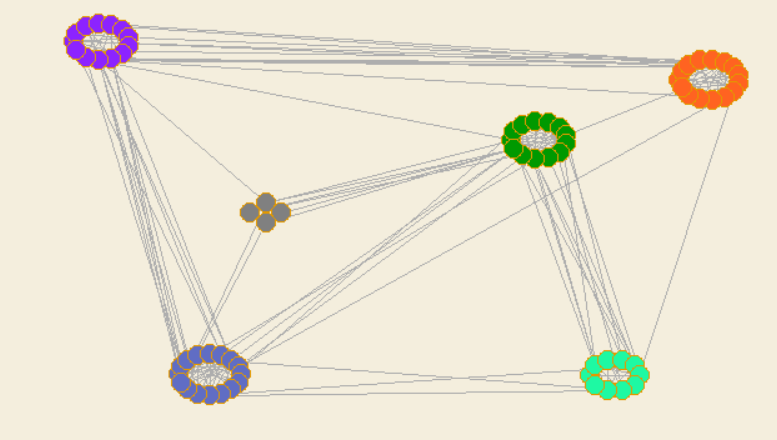
\includegraphics[width = 0.7\textwidth]{figs/pajek-ex2.png}
\end{figure}

\section{Neo4j}
Neo4j es la base de datos orientada a grafos que más se utiliza. Puede utilizar grafos dirigos y no dirigidos, grafos ponderados (con una unidad en el arco), grafos con etiquetas (los nodos y los arcos pueden tener propiedades). Todos estos se pueden manejar en Neo4j, recibiendo el nombre de grafos de propiedad. Las ventajas de esta base de datos es su alto rendimiento, su gran agilidad (facilidad para añadir propiedades, nodos, relaciones, etc.) y su gran flexibilidad y escalabilidad. 

Dos casos de uso de esta base de datos es la detección de fraude de tarjetas para pagos online y recomendaciones en tiempo real y redes sociales. Comparando una base de datos relacional con una base de datos basada en grafos, los términos se traducirían de la siguiente forma:
\begin{table}[htbp]
\centering
\begin{tabular}{l l}
Base de datos relacional & Base de datos de grafos \\ \hline
Tablas & Grafos \\
Filas & Nodos \\
Columnas y datos & Propiedades y sus valores \\
Limitaciones & Relaciones \\
Joins & Traversal o recorridos.
\end{tabular}
\end{table}

Neo4j utiliza el lenguaje de consulta CQL (Cypher Query Language). Utiliza grafos de propiedades con índices que permiten acelerar las operaciones. Se pueden utilizar restricciones con UNIQUE, y sigue el modelo ACID de las bases de datos tradicionales. Hay una interfaz para ejecutar comandos CQL. Los grafos se almacenan de forma nativa, es decir, los nodos cercanos en el grafo se almacenan de forma contigua en el disco. Los comandos de consulta se pueden ejecutar desde Java, Spring, Scala, etc. 

\subsection{Modelo de datos}
El modelo de datos es un grafo con nodos, propiedades y etiquetas. Un nodo muestra cada registro, pudiendo tener propiedades en formato de pares nombre-valor que pueden contener cadenas, números o booleanos. Las etiquetas son una forma de agrupar nodos similares (equivalente a las clases en la programación orientada a objetos). Las relaciones siempre tienen dirección (todos los grafos son dirigos) y tienen un tipo. Además, pueden tener propiedades. 

\begin{figure}[htbp]
\centering
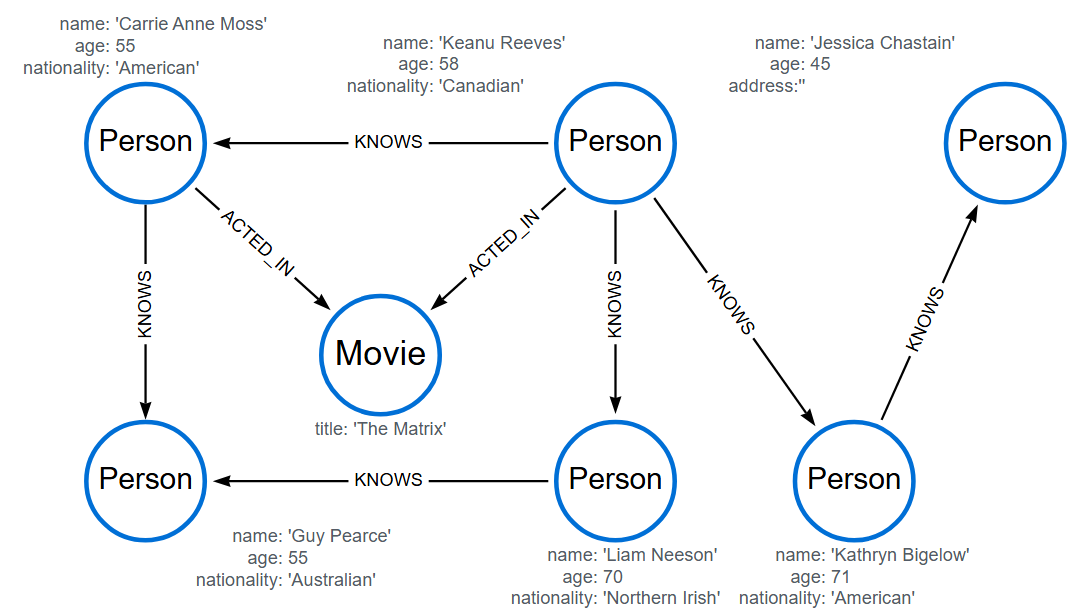
\includegraphics[width = 0.8\textwidth]{figs/neo4j-graph.png}
\end{figure}

\subsection{Lenguaje de consulta Cypher (CQL)}
CQL utiliza patrones para describir los datos, por lo que se conoce como lenguaje de pattern-matching. La sintaxis es sencilla y legible, teniendo cláusulas parecidas a SQL: comandos para insertar y borrar, cláusulas como WHERE y ORDER BY, funciones para cadenas, funciones agregadas, etc.
\begin{itemize}
\item CREATE: para crear nodos, relaciones y propiedades
\item MATCH: para conseguir datos sobre nodos, relaciones y propiedades
\item RETURN: para obtener los resultados de las consultas.
\item WHERE: dar condiciones para filtrar los datos obtenidos
\item DELETE: borrar nodos y relaciones
\item REMOVE: borrar propiedades de nodos y relaciones
\item ORDER BY: ordenar los datos obtenidos
\item SET: añadir o actualizar etiquetas
\end{itemize}

El comando CREATE \marginpar[\footnotesize CREATE]  \ sirve para crear nodos con y sin propiedades, relaciones con y sin propiedades, y etiquetas para nodos y relaciones. La sintaxis es CREATE(<node-name>:<label-name>), por ejemplo, \texttt{CREATE (:Person)} o \texttt{CREATE(p:Person)}. Las propiedades se especifican entre llaves: \texttt{CREATE (ee:Person {name:'Emil', from:'Sweden'})}. Un nodo puede tener varias etiquetas, por ejemplo \texttt{CREATE (e1:Estudiante:Person)}.

El comando MATCH \marginpar[\footnotesize MATCH \\ RETURN]  \ sirve para localizar datos sobre nodos, relaciones y propiedades. Por ejemplo, para buscar todos los nodos de tipo Person, habría que poner \texttt{MATCH(:Person)} seguido de un RETURN. El RETURN sirve para devolver propiedades sobre nodos, relaciones y propiedades, por lo que debe ir siempre con MATCH o CREATE. El comando completo especificando propiedades sería \texttt{MATCH (ee:Person) WHERE ee.name = 'Emil' RETURN ee;} y sin propiedades \texttt{MATCH (p:Person) RETURN p}. Para mostrar todo el contenido de la base de datos (nodos, relaciones y propiedades), se debe poner \texttt{MATCH(n) RETURN n}. RETURN permite crear alias con AS y obtener resultados únicos con DISTINCT. 

Se puede crear una nueva relación entre dos nodos que no existen de la siguiente forma: \texttt{CREATE p = (juan:Person {name:'Juan'})-[:TRABAJA\_EN]->(eps:Empresa{name:'EPS'}) <- [:TRABAJA\_EN]-(laura:Person{name:'Laura'}) RETURN p}.

La cláusula WHERE \marginpar[\footnotesize WHERE]  \ funciona de forma muy similar a SQL: \\
\texttt{MATCH (p1:Person) \\ WHERE p1.name = 'Allison' \\ RETURN p1} \\
\texttt{MATCH (p:Person) \\ WHERE p.name = 'Ian' OR p.name = 'Rik' \\ RETURN p}

\begin{figure}[htbp]
\centering
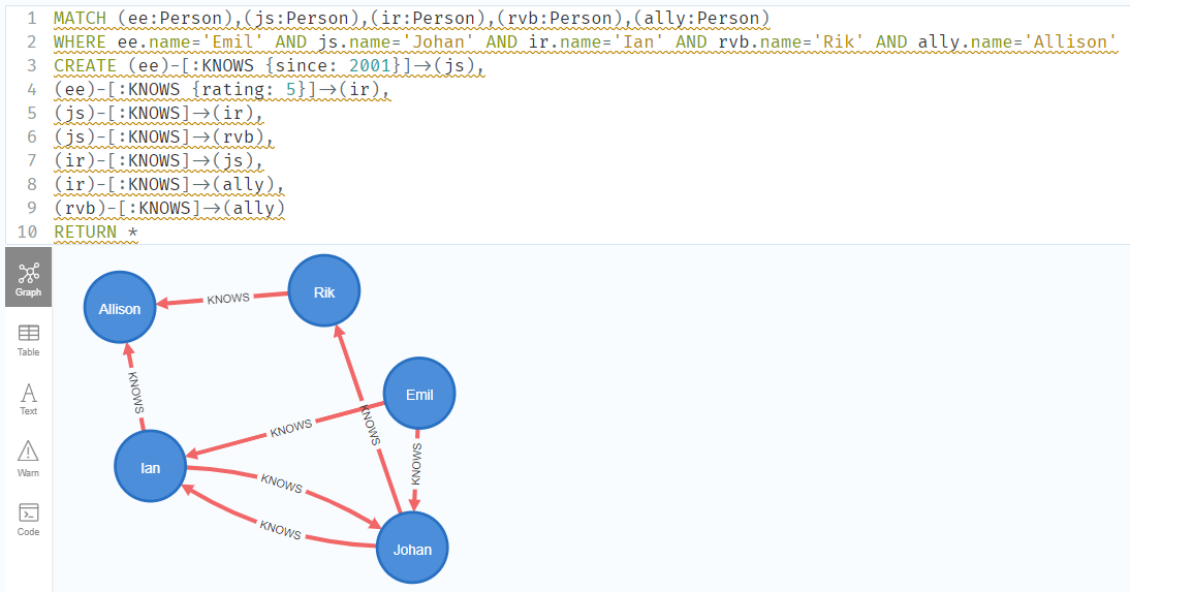
\includegraphics[width = \textwidth]{figs/where-cql.png}
\end{figure}

Para borrar \marginpar[\footnotesize DETACH DELETE \\ REMOVE]  \ toda la base de datos, se debe ejecutar \texttt{MATCH(n) DETACH DELETE n}. Para borrar una propiedad o una etiqueta de un nodo o relación, se debe utilizar REMOVE. 

SET permite \marginpar[\footnotesize SET \\ ORDER BY]  \ asignar valores a propiedades. ORDER BY funciona como en SQL, ordenando de forma ascendente de forma predeterminada.

La cláusula UNION \marginpar[\footnotesize UNION]  \ permite combinar varias consultas. UNION ALL mantiene las filas duplicadas. 

A la hora de seleccionar datos \marginpar[\footnotesize LIMIT \\ SKIP]  \ , se pueden mostrar un cierto número de filas (LIMIT x) o saltar x filas (SKIP x). 

CREATE no comprueba \marginpar[\footnotesize MERGE \\ IS (NOT) NULL]  \ si el nodo ya existe. Para que esto no ocurra, se puede utilizar MERGE. En caso de no especificar propiedades, se rellenan con null. Posteriormente, se puede acceder a ellas mediante IS NULL o eliminarlas con IS NOT NULL.

Hay varias funciones para strings: toUpper convierte todo en mayúscula, toLower en minúscula. substring permite obtener un fragmento de una cadena. El índice empieza en 0.

Neo4j permite cargar un fichero csv \marginpar[\footnotesize LOAD CSV]  \ con los datos mediante el comando \texttt{LOAD CSV WITH HEADERS FROM "file:/estudiantes.csv" AS csvLine \\ CREATE (e:Estudiante {id:toInteger(csvLine.id), nombre:csvLine.nombre})}.

%14/11 - Estrella Pulido
Las funciones agregadas permiten realizar cálculos con determinadas columnas de una tabla. Las funciones disponibles son:
\begin{itemize}
\item COUNT: devuelve el número de filas devueltas por MATCH. Se puede combinar con DISTINCT para contar los valores únicos y no todos. 
\item MAX: devuelve el valor más alto de una serie de filas 
\item MIN: devuelve el valor más bajo de un conjunto de filas
\item SUM: devuelve la suma de todas las filas 
\item AVG: devuelve la media de todas las filas
\end{itemize}

Las funciones para relaciones tienen la siguiente estructura: \texttt{CREATE (startnode) - [relationship] -> (endnote)}. Como las relaciones siempre están dirigidas, startnode es el nodo del que parte la relación y endnode donde termina. Además, a la hora de realizar las consultas, se puede omitir la dirección para obtener los resultados en ambas direcciones.

\subsubsection{Patrones y reconocimiento de patrones}
El reconocimiento de patrones (o pattern matching) pone un patrón en la consulta, describiendo la forma de lo que se busca para los caminos que se quieren encontrar. El patrón sirve para encontrar, pero lo que se devuelve se especifica en el return. 

Se pueden escribir patrones para nodos, añadiendo propiedades o para caminos. También se pueden escribir patrones para relaciones, añadiendo propiedades, pudiendo omitir el nombre de la relación o utilizando variables. Además, se puede especificar la longitud (\texttt{(a) - [*2]-> (b)}) o mantenerla variable: entre dos longitudes (\texttt{(a) - [*2::4]-> (b)}), de una longitud o más (\texttt{(a) - [*2..]-> (b)}), de una longitud o menos (\texttt{(a) - [*..4]-> (b)}) o de cualquier longitud (\texttt{(a) - [*]-> (b)}).

En los grafos, hay un algoritmo que permite encontrar el camino más corto entre dos nodos. En Neo4j, la función es \texttt{shortestPath}. Esto saca la primera opción que encuentre, pero si hubiese varios caminos de la misma longitud, se pueden mostrar con \texttt{allShortestPaths}. Es recomendable especificar una longitud máxima del camino para que el algoritmo no se eternice, sobre todo cuando el grafo es grande. 